\documentclass[12pt]{article}

\usepackage[spanish, es-tabla, es-nodecimaldot]{babel}
\usepackage[utf8x]{inputenc}
\usepackage{amsmath}

\usepackage{hyperref}
\usepackage{url}
\usepackage{textcomp}
\usepackage{gensymb}
\usepackage[dvipsnames]{xcolor}

\usepackage{parskip}
\usepackage{fancyhdr}
\usepackage{multicol}
\usepackage{vmargin}
\usepackage{setspace}
\usepackage{geometry}

\usepackage{float}
\usepackage{array}
\usepackage{graphicx}
\graphicspath{{images/}}
\usepackage{wrapfig}
\usepackage{caption}
\usepackage{subcaption}

\setmarginsrb{2 cm}{1 cm}{2 cm}{1.5 cm}{0.5 cm}{1 cm}{1 cm}{1 cm} %{izq}{up}{der}{down}{Encabezado}
\title{Equivalente Mecánico del Calor.}
\author{Martín Alejandro Paredes Sosa}		

\makeatletter
\let\thetitle\@title
\let\theauthor\@author
\let\thedate\@date										
\makeatother

\pagestyle{fancy}
\fancyhf{}
%\rhead{Lic.. Física}
%\lhead{Informe 5: \thetitle}
\cfoot{\thepage}

\begin{document}
%===================================================================================================
%====================================Titulo y Nombre================================================
%===================================================================================================
\begin{center}
{ \large \bfseries \thetitle}
\end{center}
	\begin{minipage}{\textwidth}
		\begin{center} 
			\theauthor 
		\end{center}
\end{minipage}
%===================================================================================================
\begin{abstract}
	En esta experiencia de laboratorio, se utilizo el ``\textit{El aparato del equivalente mecánico del calor}'', el cual tiene un sensor de temperatura(termistor), con el cual se midió el cambio de la temperatura de un cilindro de aluminio incrustado en el aparato. Para medir el cambio en la temperatura, se giró la manivela, para que el cilindro rozara con hilo nylon que lo envolvía y que se ato a un contrapeso. El objetivo es obtener un valor numérico del equivalente mecánico del calor.

\end{abstract}
\vspace{-1cm}
%===================================================================================================
\section{Introducción}
\vspace{-0.5cm}
Históricamente, tomo mucho tiempo en entender cuál era la naturaleza del calor. En un principio se pensó que este era un fluido, denominado calórico, que impregnaba los cuerpos y era responsable del calor que estos intercambiaban al estar en contacto. Para el siglo XIX, Joule ideó un experimento, donde demostraba que el calor era una forma de energía y que se podía obtener a partir de la energía mecánica. Joule se propuso demostrar que se podía elevar la temperatura del agua transfiriéndole energía mecánica. Este experimento se le conoce como ``experimento de Joule'' en el cual se determino el equivalente mecánico del calor.

\hspace{0.5cm}Antes del experimento, se pensaba que calor y energía eran dos magnitudes diferentes, por lo que las unidades en las que se median eran distintas. El calor se medía en con la caloría y la energía en joules. Una caloría se define como la cantidad de calor necesaria para elevar la temperatura de un gramo de agua destilada desde 14.5ºC a 15.5ºC. El descubrimiento de Joule llevó a la teoría de la conservación de la energía lo que a su vez condujo al desarrollo del primer principio de la Termodinámica.

\hspace{0.5cm} Esta experiencia en el laboratorio consistió en utilizar el ``\textit{El aparato del equivalente mecánico del calor}''. Este instrumento nos permite obtener la temperatura de un cilindro de aluminio incrustado al aparato, a partir de su resistencia. Cuando se gira la manivela, el cilindro roza con hilo nylon generando un cambio en la temperatura del cilindro. El objetivo de este experimento, es demostrar los cambios en la energía mecánica a la energía en forma de calor y así tener un valor numérico del equivalente mecánico del calor.
\pagebreak

%===================================================================================================
\section{Desarrollo Experimental}\vspace{-0.5cm}
Primeramente, se investigó la capacidad calorífica del aluminio. Para empezar con el experimento se midió la masa del cilindro y del contrapeso y luego las dimensiones del cilindro.

\begin{figure}[H]
\centering
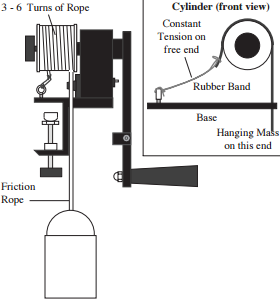
\includegraphics[width=0.35\linewidth ]{arregloS.png}
\caption{Arreglo Experimental}
\label{fig:Arreglo}
\end{figure}

Una vez que se termino de medir el cilindro, se coloco en el refrigerador hasta que alcanzara una temperatura 10°C por debajo de la temperatura de la habitación. Una vez que se alcanza dicha temperatura se monta rápidamente sobre el aparato. Para montarlo, se debe insertar el cilindro al aparato y se le pone polvo de grafito, luego se enrolla con el hilo nylon dando 5 vuelta aproximadamente. El grafito se utiliza para que la cuerda se deslice sobre el cilindro. Una vez enrollado se procede a colocar el contrapeso a una distancia aproximada de 3 cm del suelo. Al mismo tiempo se conecto el termistor a la interfaz PASCO, la cual se configuro para utilizar el termistor.

Ya colocado el sistema, se tomo la temperatura ambiente y la del cilindro y se procedió girar la manivela a una velocidad constante. Cuando el cilindro alcanzo una temperatura de 10°C por arriba de la habitación, se dejo de girar. Se tomo nota del numero de vueltas y la temperatura final.

Se removió el cilindro y se metió al refrigerar nuevamente para repetir el experimento.
\pagebreak
%===================================================================================================
\section{Resultados}
La tabla \ref{tab:Med} muestra las mediciones que se realizaron antes de empezar el experimento.

	\begin{table}[H]
		\centering
		\begin{tabular}{|c|c|}
			\hline
			\textbf{Medición}				  & \textbf{Valor} 				  \\ \hline
			Temperatura ambiente 			  & 24.1 $\pm$ 0.21 °C 			  \\ \hline
			Calor Especifico Aluminio ($C_c$) & 0.22 $\frac{cal}{g\celsius}$  \\ \hline
			Diámetro Cilindro 				  & 4.94 $\pm$ 0.002 cm			  \\ \hline
			Masa Cilindro ($m$)				  & 204.23$\pm$ 0.002 g			  \\ \hline
			Masa Contrapeso ($M$)			  & 4.38 $\pm$ 0.002 kg			  \\ \hline
		\end{tabular}
		\caption{Mediciones Previas al Experimento.}
		\label{tab:Med}
	\end{table}


Para obtener el trabajo que se suministro al cilindro cuando se gira la manivela es igual al torque $\tau$ que actúa en el, por angulo ($\theta$) sobre el cual el torque actúa. No es sencillo calcular el torque de la manivela, pero , como el movimiento del cilindro es aproximadamente constante, se sabe que el torque de la palanca debe balancear el torque que proviene de la fricción de la cuerda. Este se calcula:
\begin{equation}
\label{Eq:Torque}
\tau = MgR
\end{equation}

donde $M$ es la masa del contrapeso, $g$ la aceleración de la gravedad y $R$ el radio del cilindro. Cada vuelta completa, el torque aplicado sobre el cilindro por un ángulo de 2$\pi$. El trabajo total aplicado es:
\begin{equation}
\label{Eq:Work}
W=\tau\theta = MgR(2\pi N)
\end{equation}
con N siendo el numero de vueltas.

Utilizando la ecuación \eqref{Eq:Work} se genero la siguiente tabla:
	\begin{table}[H]
		\centering
		\begin{tabular}{|c|c|c|}
			\hline
			\textbf{Medición} &\textbf{Vueltas} & \textbf{Trabajo $W$} \\ \hline
			1 & 574 & 3827.65 $\pm$ 0.002 J \\ \hline
			2 & 519 & 3460.89 $\pm$ 0.002 J \\ \hline
			%3 & 707 & 4733.63 $\pm$ 0.002 J \\ \hline
		\end{tabular}
		\caption{Calculo del Trabajo Realizado.}
		\label{tab:WORK}
	\end{table}

Para calcular el calor generado por fricción, se determina midiendo el cambió en la temperatura. El calculo es el siguiente:
\begin{equation}
\label{Eq:Calor}
Q = mC_c(T_f-T_0)
\end{equation}

Donde $m$ es la masa del cilindro, $C_c$ el calor especifico del aluminio y $T_f$ y $T_0$ son la temperatura final e inicial respectivamente.

Utilizando la ecuación \eqref{Eq:Calor} se genero la siguiente tabla:
	\begin{table}[H]
		\centering
		\begin{tabular}{|c|c|c|c|}
			\hline
			\textbf{Medición} &\textbf{Temperatura $T_0$ } & \textbf{Temperatura $T_f$ }& \textbf{Calor $Q$} \\ \hline
			1 & 13.8 $\pm$ 0.36\celsius & 35.0 $\pm$ 0.36\celsius & 952.53 $\pm$ 0.362 cal \\ \hline
			2 & 17.1 $\pm$ 0.36\celsius & 36.2 $\pm$ 0.36\celsius & 858.17 $\pm$ 0.362 cal \\ \hline
			%3 & 19.5 $\pm$ 0.36\celsius & 35.3 $\pm$ 0.36\celsius & 709.90 $\pm$ 0.362 cal \\ \hline
		\end{tabular}
		\caption{Calculo del Trabajo Realizado.}
		\label{tab:Calor}
	\end{table}

Conocidos estos valores, se puede calcular el equivalente mecánico del calor ($J$). $J$ es la relación entre el trabajo y el calor.
\begin{equation}
\label{Eq:J}
J = \frac{W}{Q}
\end{equation}

Utilizando la ecuación \eqref{Eq:J} se genero la siguiente tabla:
	\begin{table}[H]
		\centering
		\begin{tabular}{|c|c|c|c|}
			\hline
			\textbf{Medición} & \textbf{Trabajo $W$ } & \textbf{Calor $Q$ } & \textbf{Equivalente $J$} \\ \hline
			1 & 3827.65 $\pm$ 0.002 J & 952.53 $\pm$ 0.362 cal & 4.02 J/cal \\ \hline
			2 & 3460.89 $\pm$ 0.002 J & 858.17 $\pm$ 0.362 cal & 4.03 J/cal \\ \hline
			%3 & 4733.63 $\pm$ 0.002 J & 709.90 $\pm$ 0.362 cal & 6.67 \\ \hline
			\multicolumn{3}{|c|}{\textbf{Promedio}}            & 4.03 J/cal \\ \hline
		\end{tabular}
		\caption{Calculo del Trabajo Realizado.}
		\label{tab:J}
	\end{table}



%===================================================================================================
\section{Discusión} 
Se llego a que la equivalencia entre unidades de calor y energía es 4.03 J/cal mientras los textos nos dicen que dicho valor es de 4.18 J/cal. Por lo tanto, el experimento nos da una buena aproximación del equivalente mecánico del calor, de hecho se tiene un 3.71\% de error. Este valor se ha calculado con diversos experimentos, y con este experimento se obtuvo un buen resultado.

%===================================================================================================
\section{Conclusiones}
Se llegó a que existe una relación entre la energía mecánica y el calor, ya que se observó que existe un aumento en la temperatura del cilindro cuando este gira. A este aumento se le atribuye a la fricción entre la cuerda y el cilindro. Llegamos a que 1 caloría equivale un aproximado de 4.03 J, lo que nos deja a un valor muy cercano al encontrado en los libros. 
%================================================================================================


\begin{thebibliography}{3}
	\bibitem{acu}
		Acuña, H. (2015). \textit{Manual de Guías de Experiencias en el Laboratorio de Termodinámica Clásica}.

	\bibitem{Joule}
		Serrano Fernandez, A., Martín Blas, T. (s.f.) \emph{Equivalente mecánico del calor} Recuperado el 14 de Mayo de 2017 de \url{http://acer.forestales.upm.es/basicas/udfisica/asignaturas/fisica/termo1p/joule.html}
	
	\bibitem{Pasco}
		Pasco (s.f.) \textit{Mechanical Equivalent of Heat} Recuperado el 14 de Mayo de 2017 de \url{www.pasco.com}
\end{thebibliography}
%================================================================================================

\end{document}

